% !TEX TS-program = XeLaTeX
% !TEX spellcheck = en-US
\documentclass[aspectratio=169]{beamer}

\usetheme{bi}

\title{Lecture 3:\\ LDA and regularised regression analysis}
\institute{GRA4160: Predictive modelling with machine learning}
\date{January 25th 2023}
\author{Vegard H\o ghaug Larsen}

\begin{document}

\maketitle

\frame{
	\frametitle{Plan for today:}

	\begin{enumerate}
		\item Linear discriminant analysis
		\item Regularised regression analysis
		\item Exercise: Predicting house prices
	\end{enumerate}
}

\frame{
	\frametitle{Linear discriminant analysis}
	\begin{itemize}
		\item Linear discriminant analysis (LDA) is a classification method
		\item LDA finds a linear combination of the features that maximizes the separation between classes
		\item Assumptions for LDA:
		\begin{enumerate}
			\item The classes are normally distributed
			\item The classes have the same covariance matrix
			\item The classes are linearly separable
		\end{enumerate}
		\item We will look at how this can be implemented in Scikit-learn
	\end{itemize}
}

\frame{
	\frametitle{Regularised regression analysis}
	\begin{itemize}
		\item A type of regression analysis that penalizes large coefficients to prevent overfitting.
		\pause
		\item Achieved by adding a penalty term to the cost function that is being optimized.
		\pause
		\item We will look at:
		\begin{enumerate}
			\item Ridge regression
			\item Lasso regression
			\item Elastic net regression
		\end{enumerate}
	\end{itemize}
}

\frame{
	\frametitle{Ridge regression}
	\begin{itemize}
		\item Ridge regularization use the L2-norm to penalize the coefficients
	\end{itemize}

	\pause

	The cost function for Ridge Regression is defined as:

	\[ J^{\text{ridge}}(\mathbf{\beta}) = \frac{1}{2n}\sum_i\left(y_i - \beta_0 - \sum_j\beta_jx_{ij}\right)^2 + \lambda_r \sum_j\beta_j^2 \]
}

\frame{
	\frametitle{Lasso regression}
	\begin{itemize}
		\item Lasso regularization use the L1-norm to penalize the coefficients
		\item Can calculate the full regularization path for all values of $\lambda$ for a given dataset using the LARS algorithm
	\end{itemize}

	\pause

	The cost function for Lasso Regression is defined as:

	\[ J^{\text{lasso}}(\mathbf{\beta}) = \frac{1}{2n}\sum_i\left(y_i - \beta_0 - \sum_j\beta_jx_{ij}\right)^2 + \lambda_l \sum_j|\beta_j| \]
}

\frame{
	\frametitle{Estimation picture for lasso and ridge}
	% insert picture here
	\begin{center}
		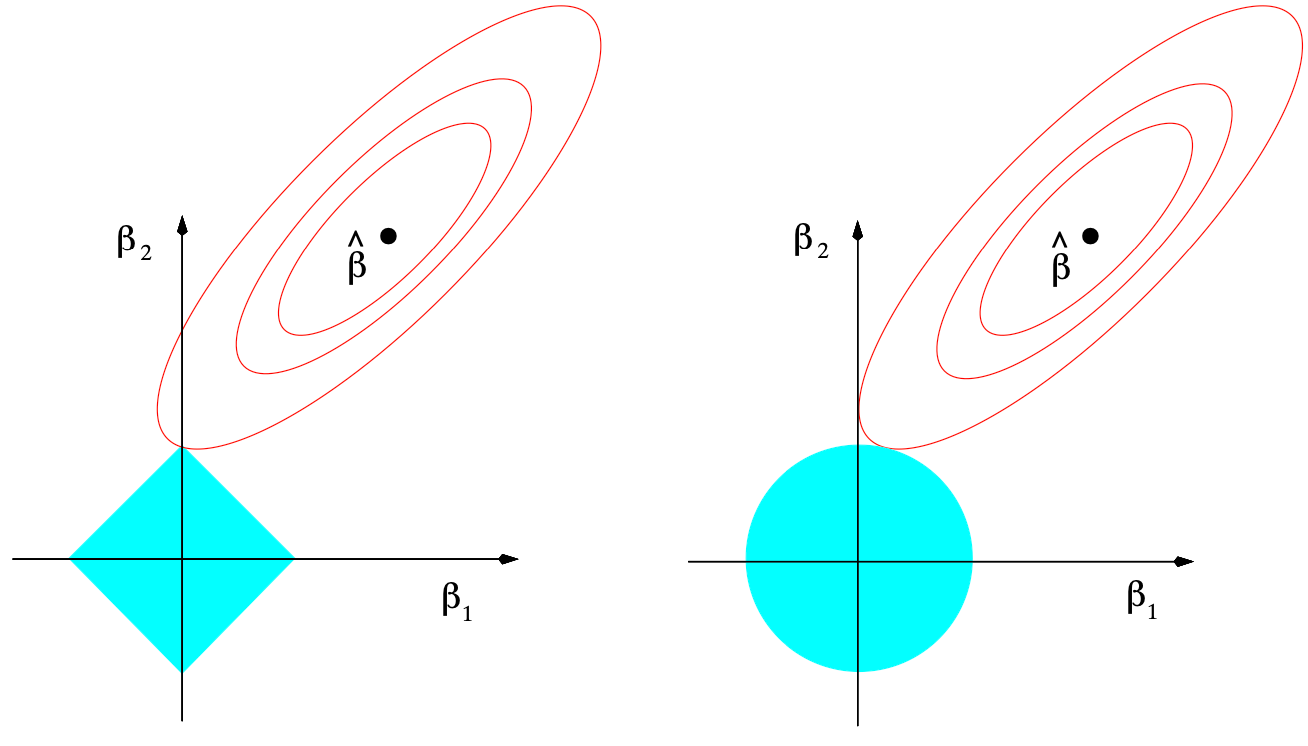
\includegraphics[scale=0.23]{figures/Estimation_picture.png}
	\end{center}
	Source: Hastie, Tibshirani and Friedman (2009)
}


\frame{
	\frametitle{Elastic net regression}
	Elastic net regularization is a combination of ridge and lasso regularization.

	\pause

	The cost function for Ridge Regression is defined as:

	\[J^{\text{elastic net}}(\mathbf{\beta}) = \frac{1}{2n}\sum_i\left(y_i - \beta_0 - \sum_j\beta_jx_{ij}\right)^2 + \lambda_{e} \left( (1-\alpha)\sum_j \beta_j^2 + \alpha \sum_j|\beta_j|\right)\]
}

\frame{
	\frametitle{Exercise: Predicting house prices}

	\begin{enumerate}
		\item Do some data cleaning and preprosessing
   		\item Train a model for predicting the house price using a linear, ridge and lasso model.
		\item Identify the most important features for the model
		\item Experiment with how changing the inputs affect the predicted price.
	\end{enumerate}
}

\end{document}